\subsubsection{Iteration}
\label{section:perf-iteration}

The first relevant test suite for investigating the performance regarding iteration is the \texttt{primal(n)} test suite, the performance of which is shown in \autoref{figure:primal-mips}.

\begin{figure}[H]
    \centering
    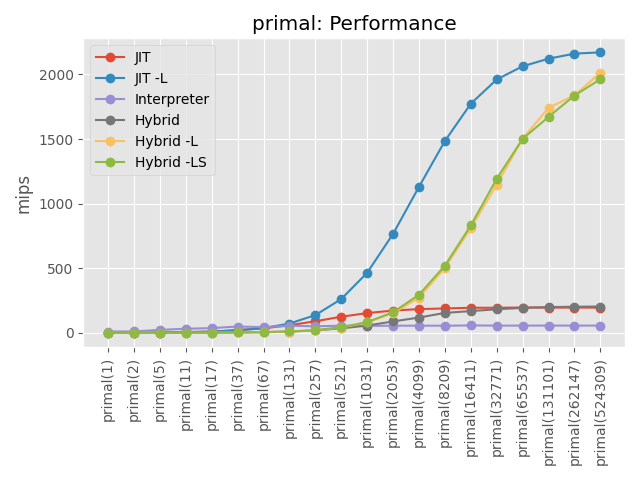
\includegraphics[scale=0.75]{output/graphs/tests/all/primal/mips.png}
    \caption{Performance in mips of the primal test suite.}
    \label{figure:primal-mips}
\end{figure}

Despite the relatively low performance across the board for low \texttt{n}, we see that the performance sky rockets for the JIT and hybrid emulators with \texttt{-L} enabled as \texttt{n} increases, before plateuing above a staggering 2000 mips. Without \texttt{-L} enabled, the peak performance is an order of magnitude higher, yet they still far exceed the performance of the interpreter, which appears to see little to no improvement as \texttt{n} increases.

\autoref{figure:primal-time} shows the execution time of the same test suite, yielding us a different perspective on the performance characteristics. We see that the interpreter is able to achieve extremely low execution times at low \texttt{n}, as low as $\sim1\si{\micro\second}$. As \texttt{n} increases, the exeuction time is directly proportional to \texttt{n}. This shows that the performance of the interpreter is relatively constant, seeing little change with \texttt{n}; the extremely low execution time floor is indicative of the interpreter's minimal overheads and thus suitability to small workloads.

\begin{figure}[H]
    \centering
    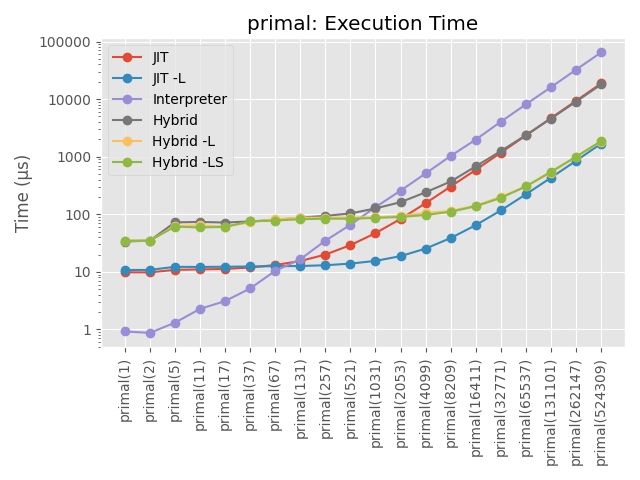
\includegraphics[scale=0.75]{output/graphs/tests/all/primal/time.png}
    \caption{Execution time of the primal test suite.}
    \label{figure:primal-time}
\end{figure}

The JIT emulator shows quite a different curve. It remains constant at $\sim10\si{\micro\second}$ for about half of the test suite, indicative of its high overhead and low initial performance. For these values of \texttt{n}, the added work is insignificant to the initial overhead and thus we see continually increasing performance. As \texttt{n} becomes sufficiently large, we see the execution time of the JIT emulator become proportional to \texttt{n}, showing that the overhead is no longer the dominating factor. We can see that both the hybrid and JIT emulator's converge to the same curve, regardless of \texttt{-L} being enabled or not, suggesting that both emulators have the same `steady state' peak performance under this workload.

The hybrid emulator displays its signature behaviour of acting like the interpreter for low \texttt{n}, after which it acts more like the JIT emulator.

The underlying reason for these performance characteristics is clear; higher \texttt{n} leads to more intensive iteration, which in turn leads to hotter programs. The results observed here closely match with how the emulators respond to hotness, as explored in \Cref{section:perf-interpreter,section:perf-jit,section:perf-hybrid}. Furthermore, the \texttt{primal(n)} test suite is extremely arithmetic heavy with no memory operations, allowing the JIT and hybrid emulators to achieve extremely high performance with \texttt{-L} enabled. It is clear that the JIT significantly outperforms the interpreter for arithmetic and iteration heavy workloads.

The next test suite to investigate is the \texttt{unroll(n/m)}; unlike the other test suites explored, the amount of functional work in all tests is fixed. The test contains a loop with \texttt{n} iterations, unrolled into chunks of size \texttt{m}. In other words, when $m=n$, no unrolling is performed and we have a single instance of the loop, iterating \texttt{m} times. Likewise, when $m=1$, the loop is fully unrolled into a single instance with no iterations. As \texttt{m} increases, the program becomes more iterative, whilst keeping the amount of actual work relatively fixed.

\begin{figure}[H]
    \centering
    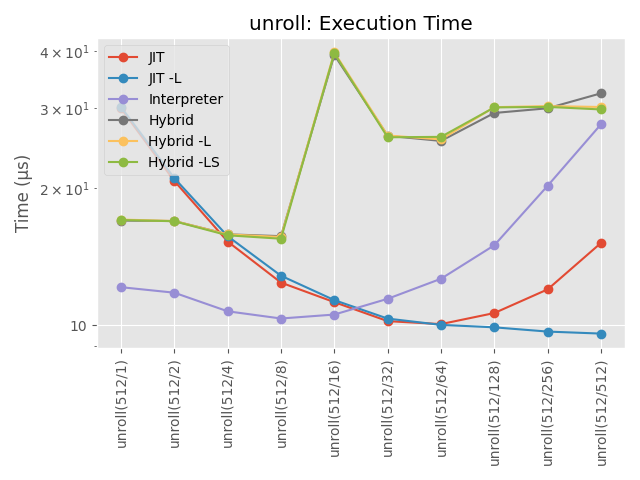
\includegraphics[scale=0.75]{output/graphs/tests/all/unroll/time.png}
    \caption{Execution time of the unroll test suite.}
    \label{figure:unroll-time}
\end{figure}

The execution times of the test suite is shown in \autoref{figure:unroll-time}; unlike other test suites, the execution time is not monotonic in all cases.

We will begin with the interpreter. As \texttt{n} increases, the unroll factor decreases and the program becomes more iterative. We can see that the execution time generally increases; the less unrolled the loop, the more branch instructions evaluated and thus the more work required by the interpreter. This also reduces the proportion of time spent by the interpreter on fast arithmetic instructions. In this sense, the interpreter behaves quite typical of how a real CPU would with an unrolled program: more unrolling generally gives higher performance.

On the other hand, the JIT emulator experiences a very different characteristic. The JIT emulator has the highest execution time when the loop is fully unrolled, and increases in performance as the loop becomes more iterative. As mentioned earlier, less unrolling leads to slightly higher total work required, as more branches need evaluating. Despite this, the JIT emulator performs better the less unrolled the program is for a simple reason; less unrolling means the source block is smaller, and less instructions are compiled. Less unrolling leads to a hotter program with a higher compilation efficiency, both of which were shown in \autoref{section:perf-jit} to increase the performance of the JIT emulator.

One peculiarity is how execution time falls monotonically with \texttt{-L} enabled, but is actually parabolic with it disabled. This is because, without \texttt{-L} enabled, a less unrolled loop would also cause a higher overhead from the runner dispatching to the host blocks each iteration, similar to how the interpreter suffered from the increased branch frequency. This becomes a trade-off with the reduced compilation overhead, and hence a sweetspot appears where the combined effect of the two opposing factors is minimised, resulting in the parabola. With \texttt{-L} enabled, the blocks are relinked and no significant overhead is introduced by the more frequent branches, and hence the sweetspot disappears. 